\section{Problema 2: Juntando piezas}

\subsection{Introducción}

En este problema, Indiana Jones y su grupo deben recorrer un conjunto de salas conectadas por paredes que se pueden romper bajo un cierto costo. El objetivo es encontrar el costo mínimo que se debe pagar para poder visitar todas las salas.

Para representar el problema, se recibe por parámetro de entrada una matriz de caracteres $M$ de $F$ filas por $C$ columnas definida de la siguiente manera, dados $i \in [0,F-1]$, $j \in [0,C-1]$:

\begin{itemize}
	\item Si $M_{ij}$ es un espacio caminable, $M_{ij} = $ '.'
	\item Si $M_{ij}$ es una pared irrompible, $M_{ij} = $ '$\#$'
	\item Si $M_{ij}$ es una pared rompible, $M_{ij}$ es un entero entre $1$ y $9$ que representa el costo de romper dicha pared.
\end{itemize}

También sabemos por enunciado que los caracteres del borde del mapa corresponden a una pared irrompible. Lo que quiere decir que $i \in \{0, F-1\} \ \vee \ j \in \{0, C-1\} \Rightarrow M_{ij} =\ $'$\#$'.

Los movimientos que se pueden realizar son horizontales o verticales y solo se puede ir desde un espacio caminable hacia otro adyacente o hacia otro que sea vecino a una puerta rompible adyacente.

En cuanto a las puertas rompibles, solo puede haber una si esta tiene exactamente dos paredes adyacentes (independientemente de si son rompibles o no).

Para especificar formalmente el problema, vamos a definir algunos conjuntos y funciones auxiliares.

Llamaremos a los intervalos discretos $filas = [0,F-1]$ y $cols = [0,C-1]$

Dados $i_1,i_2 \in filas$ y $j_1,j_2 \in cols$ definimos la función de distancia como

$dist: filas \times cols \times filas \times cols \rightarrow \mathbb{N}_0$

$dist(i_1,j_1,i_2,j_2) = |i_1 - i_2| \quad + \quad |j_1 - j_2|$

Definimos el conjunto de movimientos posibles $P$ como aquellas posiciones que tienen distancia 1, ninguna es pared irrompible y no son ambas paredes rompibles.
\\

$P = \{(i_1,j_1,i_2,j_2) \in filas \times cols \times filas \times cols \quad | \quad dist(i_1,j_1,i_2,j_2) = 1 \quad \land \quad M_{i_1,j_1} \neq \# \quad \land \quad M_{i_2,j_2} \neq \# \quad \land \quad \lnot (M_{i_1,j_1}, M_{i_1,j_2} \in [1,9] )\}$

\vspace{1em}

Ahora, sea $costo: P \rightarrow \mathbb{N}_0$ la función de costo

$$costo(i_1,j_1,i_2,j_2) = \left\{ \begin{array}{lcc}
             				   0            &   si \quad  M_{i_2,j_2} = $ '.'$ \\
             				\\ M_{i_2,j_2}  &   sino                \\
             				\end{array}
   			 				\right.$$

Una vez formalizado el costo, queremos encontrar una secuencia $S$ de pasos $(i,j)$ que pase por todos los espacios caminables un paso a la vez y cuya suma de costos sea mínima. Es decir

\begin{align*}
& ((\forall k \in \mathbb{N}) \quad dist(S_k,S_{k+1}) = \ 1) \qquad \land  \\
& ((\forall i, j \in filas \times columnas) \quad M_{ij} = \text{'.'} \quad \Leftrightarrow \quad (\exists k \in \mathbb{N}) \quad S_k = (i,j))
\end{align*}

y, para toda secuencia $S'$ que cumple lo anterior

$$\sum_{k \in \mathbb{N}} costo(S_k,S_{k+1}) \quad \leq \quad \sum_{k \in \mathbb{N}} costo(S'_k,S'_{k+1})$$

Esto define formalmente el problema que se debe resolver en este ejercicio.

El enunciado pide, además, una solución con complejidad $\mathcal{O}(FC \times log(FC))$ donde $F$ es la cantidad de filas de $M$ y $C$ es la cantidad de columnas.

\subsection{Solución}

Elegimos representar este problema como un grafo con pesos en las aristas cuyos vértices son los espacios libres y las aristas el costo que lleva caminar de un espacio libre a otro. Entre dos vértices de espacio libre en los que hay una pared rompible en el medio, el peso de la arista que los incide es el costo de la pared en cuestión. Si no hay, entonces el costo es $0$. Cabe destacar que aquellos espacios libres que no sean vecinos o que no tengan exactamente una pared rompible en el medio no tendrán aristas que los conecten.

Esta representación es posible porque entre dos espacios libres hay siempre a lo sumo una pared rompible que los conecta, debido a la restricción del enunciado que establece que si una pared es rompible, entonces debe tener exactamente dos paredes adyacentes, lo cual implica que una pared rompible no puede conectar más de 2 salas.

Una vez establecido el grafo que representa nuestro problema, la estrategia a seguir es utilizar el algoritmo de Kruskal para encontrar un árbol generador mínimo de nuestro grafo (justificación de por qué utilizamos este algoritmo en la sección de correctitud) y la solución que se devuelve es el peso total del mismo árbol generado por Kruskal.

El pseudo-código de lo que hace el algoritmo que resuelve el problema tiene la siguiente forma:

\begin{lstlisting}
input: M : matriz<casillas>

//Primero se agregan todas las aristas del grafo en un conjunto ordenado
set<aristas> candidatos $\leftarrow$ $\emptyset$

para toda posicion $p$ que sea espacio libre en $M_p$
	crear una componente conexa con unico elemento $p$
	para cada vecino $q$ de $p$
		si $q$ es espacio libre
			agregar arista $(p,q)$ con peso $0$ a candidatos
		si $q$ es pared rompible
			buscar el espacio libre $r$ con el que conecta $q$ y agregar arista $(p,r)$ con el costo de $q$ a candidatos

//Ahora se aplica el algoritmo de Kruskal sobre el conjunto ordenado de aristas
int res $\leftarrow$ $0$
para toda arista $e$ en candidatos (recorrida por orden de peso)
	si los extremos de $e$ ($u$ y $v$) estan en diferentes componentes conexas
		unir $u$ con $v$ en una misma componente conexa
		res $\leftarrow$ res + peso(e)

si hay una sola componente conexa
	retornar res
sino
	retornar que no hay solucion
\end{lstlisting}

Cabe destacar que en el algoritmo en sí, no se crea el grafo de manera explícita, sino que se trabaja con las posiciones libres de la matriz como si ya fueran los vértices de forma implícita. El conjunto de aristas si es creado. Esto no imposibilita la representación del problema en grafos como tal ya que el algoritmo sigue siendo fiel a la idea presentada.

\subsubsection{Correctitud}

Debido a que la correctitud del algoritmo de Kruskal se asume que ya fue probada en la parte teórica de la materia, esta sección se centra en justificar por qué la representación y el algoritmo seleccionados dan una respuesta correcta al problema planteado por este ejercicio.

Retomando un poco lo mencionado en la sección de Solución, el grafo $G$ que elegimos para representar el problema es aquel cuyos vértices son los casilleros libres de la matriz y las aristas conectan los espacios libres que tienen distancia uno o una pared rompible que los separa. Si hay una pared rompible entre dichos espacios, el peso de la arista es el mismo que el costo de dicha pared, y sino, es cero.

Asumiendo que se recibe una matriz que tiene solución (es decir, existe al menos una forma de pasar por todos los casilleros vacíos) se puede ver que el grafo correspondiente resulta conexo, ya que por cada conexión entre dos casilleros hay una arista que une los vértices que representan a esos mismos casilleros.

El árbol que devuelve algoritmo de Kruskal representa un posible recorrido por la matriz donde las aristas representan los caminos que se deben seguir. Como este árbol es generador de $G$, tiene los mismos vértices que este y por ende garantiza que se recorren todos los casilleros libres, lo cual cumple una de las condiciones que debe satisfacer la solución formal del problema (mencionada en la sección de introducción).

El algoritmo de Kruskal, además, halla un árbol generador mínimo de $G$. Si el peso de las aristas representa el costo de pasar de un casillero a otro y el árbol generador mínimo es aquel que minimiza la suma total de los pesos de las aristas, entonces este mismo garantiza en su recorrido que la suma total del costo de recorrer todas las salas es el mínimo entre todos los árboles generadores de $G$. Como todas las aristas tienen peso no-negativo y un árbol generador $T$ de $G$ es un subgrafo de $G$ con cantidad minimal de aristas, agregar una arista de $G$ a $T$ significaría que su peso se volvería igual o mayor. Dicho esto, se puede concluir que para este problema, un árbol generador mínimo de $G$ posee el menor peso total entre todos los subgrafos conexos de $G$, es decir, entre todos los recorridos posibles que se pueden hacer en el mapa.

Como el algoritmo devuelve un grafo cuya representación minimiza el esfuerzo que hay que realizar para poder visitar todas las salas, queda probada su correctitud. \QEDB

\subsubsection{Complejidad}

Para entender la complejidad del algoritmo propuesto, primero hay que saber cuantos nodos tiene el grafo que elegimos para representar el problema.
Como cada nodo es una casilla de la matriz, podemos acotar la cantidad de vértices por la cantidad total de posiciones en la misma, la cual es $F \times C$. Entonces, si notamos a la cantidad de nodos de $G$ como $n$

$$n \in \mathcal{O}(FC)$$

En el algoritmo hay dos pasos bien marcados: la creación del conjunto de aristas y la aplicación del algoritmo de Kruskal.

La creación del conjunto de aristas pertenece a este fragmento:

\begin{lstlisting}
para toda posicion $p$ que sea espacio libre en $M_p$
	para cada vecino $q$ de $p$
		si $q$ es espacio libre
			agregar arista $(p,q)$ con peso $0$ a candidatos
		si $q$ es pared rompible
			buscar el espacio libre $r$ con el que conecta $q$ y agregar arista $(p,r)$ con el costo de $q$ a candidatos
\end{lstlisting}

Como puede verse, se itera un ciclo que recorre todos los casilleros de $M$ una sola vez y por cada iteración consulta sus 4 vecinos. Por cada consulta se debe hacer a lo sumo una inserción en el conjunto de aristas. Para lograr esto se utiliza la instrucción $insert$ de la estructura de datos $set$ que provee $C++$, la cual tiene complejidad logarítmica en la cantidad de elementos, o sea, $n$. En otras palabras, estamos ejecutando $\mathcal{O}(n)$ veces una operación de costo $\mathcal{O}(log(n))$, lo cual da una complejidad total de $\mathcal{O}(n \times log(n))$.

La segunda mitad del algoritmo consiste en aplicar el algoritmo de Kruskal en el grafo armado. Esto corresponde al siguiente fragmento:

\begin{lstlisting}
int res $\leftarrow$ $0$
para toda arista $e$ en candidatos (recorrida por orden de peso)
	si los extremos de $e$ ($u$ y $v$) estan en diferentes componentes conexas
		unir $u$ con $v$ en una misma componente conexa
		res $\leftarrow$ res + peso(e)
\end{lstlisting}

Por cuestiones de claridad, se presentó el pseudo-código de esta manera para ayudar al entendimiento del algoritmo por parte del lector. Sin embargo, para justificar la complejidad de este fragmento de código, es necesario hablar más detalladamente sobre el costo de las operaciones que se realizan. Estas operaciones son chequear que dos nodos estén en la misma componente conexa y, en caso contrario, unirlas. Para esto se utiliza la estructura de datos Union Disjoint Set (UDS) o también conocida como Union Find (UF), la cual sirve para manejar conjuntos disjuntos de elementos. Consta de dos operaciones: $find(x)$, que devuelve el elemento representante del conjunto al cual pertenece $x$ (lo llamaremos padre), y $union(x,y)$, que une los conjuntos a los que pertenecen $x$ e $y$ en uno solo. Existen varias implementaciones de esta estructura de datos. Nosotros elegimos la representación de listas para poder cumplir con la complejidad que pide el ejercicio.

El pseudo-código de inicializar la estructura, hacer $union$ y $find$ se presentan a continuación:

\begin{lstlisting}
$init():$
	matriz<lista<posicion>> componente
	matriz<posicion> padre
	para toda posicion $(i,j)$ que sea espacio libre en $M_{ij}$
		componente[i][j] $\leftarrow$ $\{(i,j)\}$		//lista con un solo elemento
		padre[i][j] $\leftarrow$ $(i,j)$
\end{lstlisting}

Como init recorre toda la matriz una sola vez y ejecuta instrucciones de tiempo constante, su complejidad es $\mathcal{O}(n)$

\begin{lstlisting}
$find(i,j):$
	retornar padre[i][j]
\end{lstlisting}

Es visible que la complejidad de $find$ es $\mathcal{O}(1)$

\begin{lstlisting}
$union(i_1,j_1,i_2,j_2):$
	$(i_1,j_1)$ $\leftarrow$ $find(i_1,j_1)$
	$(i_2,j_2)$ $\leftarrow$ $find(i_2,j_2)$
	si el tamanio de $componente[i_1][j_1]$ es mayor que el de $componente[i_2][j_2]$
		intercambiar $(i_1,j_1)$ y $(i_2,j_2)$
	para cada elemento $(i',j')$ de $componente[i_1][j_1]$
		$padre[i'][j']$ $\leftarrow$ $(i_2,j_2)$
		agregar $(i',j')$ a $componente[i_2][j_2]$
	vaciar $componente[i_1][j_1]$
\end{lstlisting}

Notar que siempre se recorre la lista de componentes de menor longitud. Esto será un factor clave para demostrar complejidad.

Si bien cada $union$ individual tiene un costo de $\mathcal{O}(n)$ (ya que como peor caso se debe recorrer la mitad de los elementos totales de la matriz) analicemos el costo total de hacer $n$ operaciones $union$.

Sea $p$ un elemento cualquiera de un conjunto, solo debe actualizarse si el conjunto en el que se encuentra debe unirse con un conjunto de longitud mayor o igual, por lo cual, cada vez que se actualiza $p$, el tamaño de su conjunto aumenta (como mínimo) el doble. Sabiendo esto, la cantidad máxima de actualizaciones de $p$ necesarias para que $p$ pertenezca a un conjunto de tamaño $n$ es $log_2(n)$. Por ende, para $n$ elementos, el costo total de actualizarlos a todos para unirlos en un mismo conjunto es $\mathcal{O}(n \times log(n))$.

Teniendo todos estos factores en cuenta, una versión más específica del algoritmo de Kruskal implementado es la siguiente:

\begin{lstlisting}
init()
para toda arista $e$ en candidatos (recorrida por orden de peso)
	sean $u$ y $v$ los nodos extremos de $e$
	si $find(u) \neq find(v)$
		$union(u,v)$
		res $\leftarrow$ res + peso(e)
\end{lstlisting}

Cabe destacar que cada vértice de $G$ tiene a lo sumo 4 aristas. Entonces, sea $m$ la cantidad de aristas de $G$

$$m \in \mathcal{O}(n)$$

Finalmente, como $init()$ tiene costo $\mathcal{O}(n)$ y se hacen $\mathcal{O}(n)$ operaciones $union$, el costo total de aplicar el algoritmo de Kruskal es $\mathcal{O}(n \times log(n))$

Como ambos fragmentos del algoritmo tienen complejidad $\mathcal{O}(n \times log(n))$, la complejidad total del algoritmo es:

$$\mathcal{O}(n \times log(n)) \in \mathcal{O}(FC \times log(FC))$$

lo cual cumple con la complejidad establecida por el enunciado. \QEDB

\subsection{Análisis experimental}

A continuación se presentan una serie de experimentos que ponen a prueba el algoritmo propuesto en esta sección y ayudan a mostrar que la complejidad temporal mencionada anteriormente es correcta.

Para tomar las mediciones se fabricaron casos de prueba utilizando el mismo generador de dungeons que el ejercicio 1, con la adición de que luego de generar las paredes, se convertirlas todas las paredes posibles en rompibles con un valor random entre 1 y 9 (siempre respetando las condiciones iniciales del enunciado, como por ejemplo tener exactamente dos paredes adyacentes y no ser borde).

Dado que la cantidad de operaciones que realiza el algoritmo depende de dos variables, se separa el análisis en varias secciones en las cuales se varían distintas combinaciones de las mismas.

\subsubsection{Variando $C$}

Dejando fija $F$, se obtuvieron los siguientes resultados de tiempo de ejecución en función de $C$:

\begin{figure}[H]
	\centering
	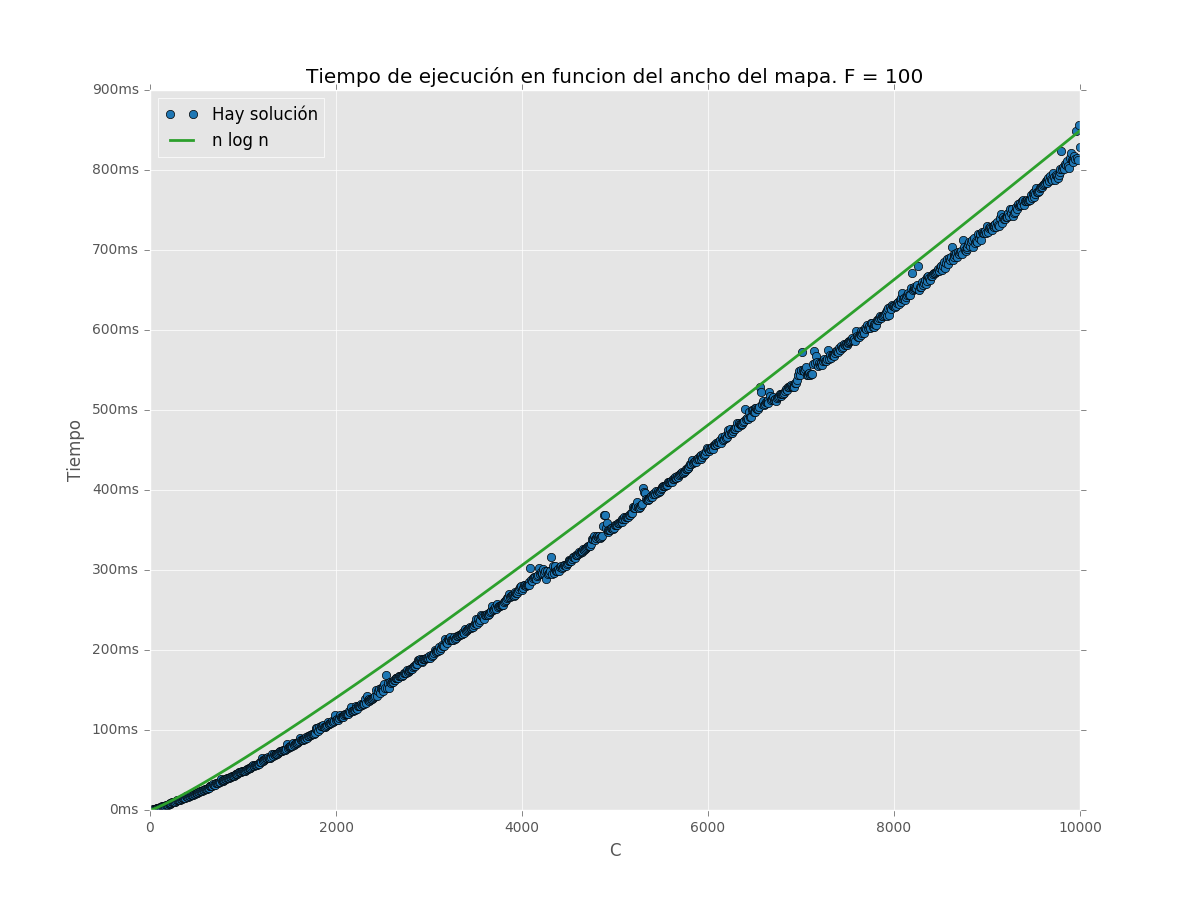
\includegraphics[width=\textwidth]{ej2-width}
	\caption{Tiempo de ejecución del algoritmo en función de $C$}
	\label{fig:ej2-width-fig}
\end{figure}

Puede observarse en la figura \ref{fig:ej2-width-fig} que todas las mediciones tomadas se encuentran acotadas por la función $n \times log(n)$, lo cual es entendible, ya que si se deja fija $F$, el algoritmo tendría complejidad $\mathcal{O}(C \times log(C))$

\subsubsection{Variando $F$}

Dejando fija $C$, se obtuvieron los siguientes resultados de tiempo de ejecución en función de $F$:

\begin{figure}[H]
	\centering
	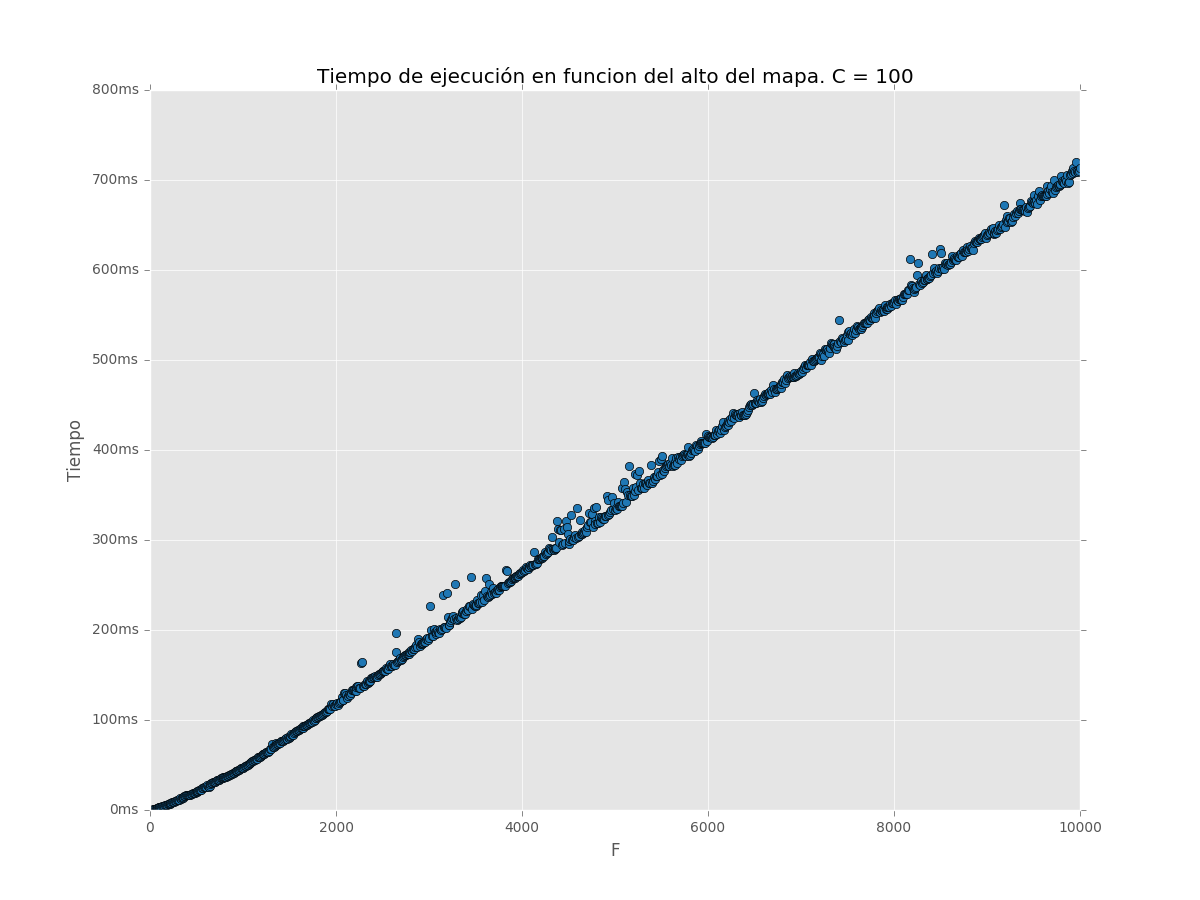
\includegraphics[width=\textwidth]{ej2-height}
	\caption{Tiempo de ejecución del algoritmo en función de $F$}
	\label{fig:ej2-height-fig}
\end{figure}

Puede observarse en la figura \ref{fig:ej2-height-fig} que todas las mediciones tomadas se encuentran acotadas por la función $n \times log(n)$, lo cual es entendible, ya que si se deja fija $C$, el algoritmo tendría complejidad $\mathcal{O}(F \times log(F))$

\subsubsection{Variando $F \times C$ de manera uniforme}

Para este experimento probamos variando $F$ y $C$ al mismo tiempo, de manera tal que se trabaja con matrices cuadradas de dimensión $F = C$ cuyo tamaño va aumentando.

\begin{figure}[H]
	\centering
	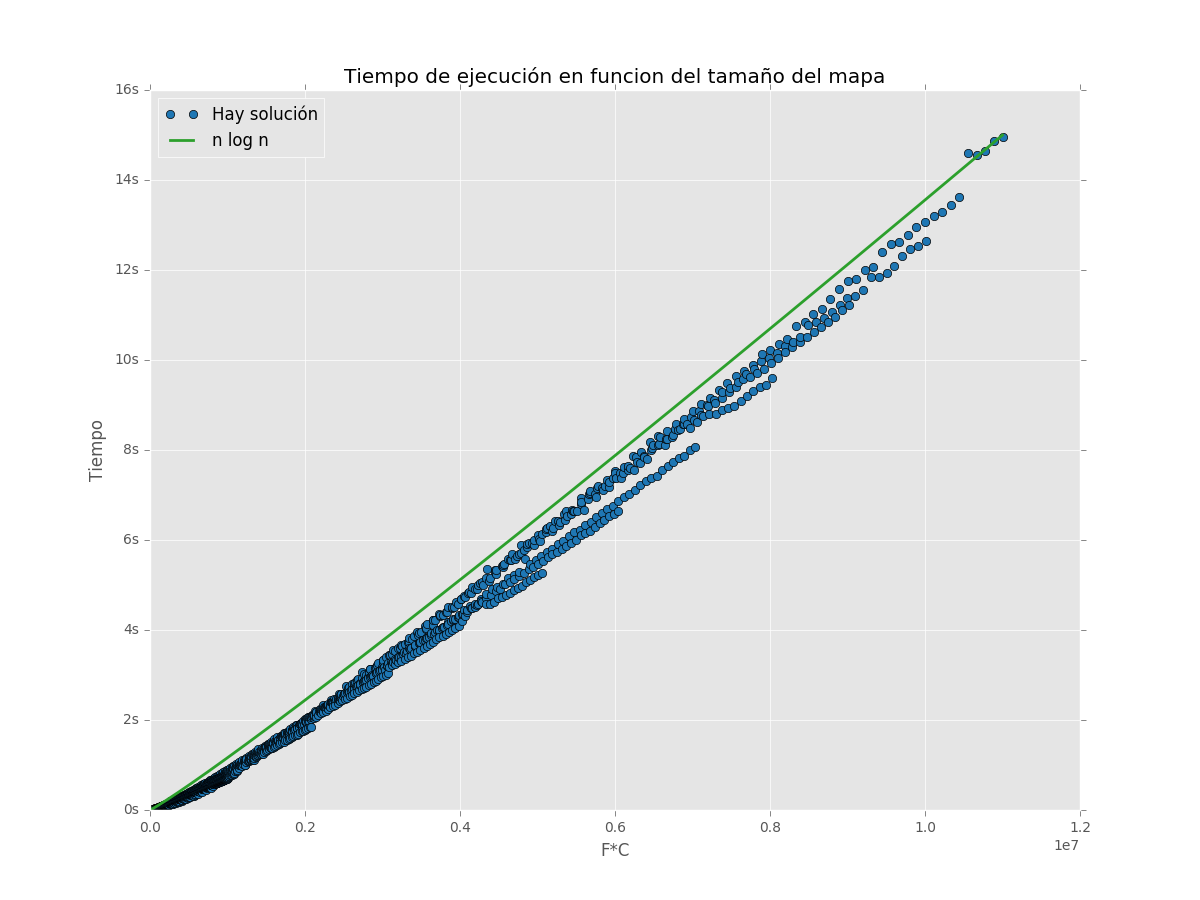
\includegraphics[width=\textwidth]{ej2-size}
	\caption{Tiempo de ejecución del algoritmo en función de $F \times C$}
	\label{fig:ej2-size-fig}
\end{figure}

Puede observarse en la figura \ref{fig:ej2-size-fig} que todas las mediciones tomadas se encuentran acotadas por la función $n \times log(n)$, lo cual evidencia aún más la complejidad $\mathcal{O}(FC \times log(FC))$ establecida en esta sección.
